\documentclass[sigconf]{acmart}

\usepackage{booktabs} % For formal tables
 \usepackage{graphicx}
 \usepackage{tabularx}
\usepackage{subcaption}

% Copyright
%\setcopyright{none}
%\setcopyright{acmcopyright}
%\setcopyright{acmlicensed}
\setcopyright{rightsretained}
%\setcopyright{usgov}
%\setcopyright{usgovmixed}
%\setcopyright{cagov}
%\setcopyright{cagovmixed}


% DOI
\acmDOI{xx.xxx/xxx_x}

% ISBN
\acmISBN{978-1-4503-5933-7/19/04}

%Conference
\acmConference[SAC'19]{ACM SAC Conference}{April 8-12, 2019}{Limassol, Cyprus} 
\acmYear{2019}
\copyrightyear{2019}


\acmArticle{4}
\acmPrice{15.00}

% These commands are optional
%\acmBooktitle{Transactions of the ACM Woodstock conference}
%\editor{Jennifer B. Sartor}
%\editor{Theo D'Hondt}
%\editor{Wolfgang De Meuter}



\begin{document}
\title{Self Healing Microservices Architecture: A case study in Docker Swarm Cluster}
%\titlenote{Produces the permission block, and
 % copyright information}
%\subtitle{Extended Abstract}
%\subtitlenote{The full version of the author's guide is available as
 % \texttt{acmart.pdf} document}


\author{Basel Magableh}
%\authornote{ }
\orcid{0000-0003-2337-637X}
\affiliation{%
  \institution{Dublin Institute of Technology}
  \streetaddress{Kevien Street}
  \city{Dublin} 
  \state{Ireland} 
  \postcode{43017-6221}
}
\email{basel.magableh@dit.ie}
 
\author{Luca Longo}
%\authornote{ }
\orcid{0000-0003-2337-637X}
\affiliation{%
  \institution{Dublin Institute of Technology}
  \streetaddress{Kevien Street}
  \city{Dublin} 
  \state{Ireland} 
  \postcode{43017-6221}
}
\email{luca.longo@dit.ie}
 
% The default list of authors is too long for headers.
\renewcommand{\shortauthors}{B. Magableh}


\begin{abstract}
Each service running in Microservices cluster could be scaled in/out based on the demand issued by end-users, orchestration algorithm, or load balancer running on the swarm manager. This means each service performance and behaviour continuously changes overtime, which makes it a challenge to use a statistical model to identify and detect anomalous behaviour in Microservices architecture. A sudden peak of the CPU some of the time could be considered to be as an anomaly as it might be an action issued by the cluster manager to meet recent high demand. The performance of the cluster nodes could fluctuate around the demand to accommodate scalability, orchestration and load balancing issued by cluster managers. This requires a model that is able to detect anomalies in real-time and generate a high rate of accuracy in detecting any anomalies and a low rate of false alarms. At the same time, it requires dynamic policy configuration that can be used to adapt the recent changes in the operational environment. This research focuses on proposing a self-healing architecture, that is the able to continuously monitor the operational environment, detects and observes anomalous behaviour, and provides a reasonable adaptation policy using multidimensional utility-based model, for self-scaling, self-healing, and self-tuning the computational resources to adapt a sudden changes in its operational environment dynamically at rune-time without human intervention.  
%This research focuses on proposing a self-healing model, that offers Microservices architecture an unsupervised anomaly detection algorithm integrated with a continuous monitoring and detection techniques that can be used to trigger adaptation strategies, which will reason about the detected anomalies and verifies the adaptation actions at runtime without human intervention.


 
  %This thesis focuses on providing a real-time unsupervised anomaly detection algorithm for microservices architecture and its implementation in Docker swarm cluster. Services running on Docker swarm are offered with load balancing and service discovery by the Docker engine. This makes it very hard to use statistical anomaly detection tools as the performance values for a service running in Docker swarm could vary based on the demand and they are continuously changing due to the dynamic load balancing and scaling offered by the Docker engine. In order to detect abnormal behaviour in a Docker swarm, it is necessary to create a model that can observe the performance of the Docker swarm cluster in real-time and provide a real-time anomaly detection based on the most recent data collected from the Docker swarm. The proposed model was implemented based on the Numenta Platform for Intelligent Computing (NUPIC). The proposed model offers anomaly detection in real-time over the streaming data found in a Docker swarm. This model is efficient and tolerant to noisy data found in streaming data with massive volumes and high velocities. Most importantly the proposed model offers continuous monitoring of real-time data and adapts to the changes in the data statistics. It also detects anomalies with a very minimum rate of false positive (false alarms).
\end{abstract}

%
% The code below should be generated by the tool at
% http://dl.acm.org/ccs.cfm
% Please copy and paste the code instead of the example below. 
%
  \begin{CCSXML}
<ccs2012>
<concept>
<concept_id>10003752.10010070.10010071.10010074</concept_id>
<concept_desc>Theory of computation~Unsupervised learning and clustering</concept_desc>
<concept_significance>500</concept_significance>
</concept>
<concept>
<concept_id>10010520.10010521.10010537.10003100</concept_id>
<concept_desc>Computer systems organization~Cloud computing</concept_desc>
<concept_significance>500</concept_significance>
</concept>
<concept>
<concept_id>10011007.10010940.10010941.10010942</concept_id>
<concept_desc>Software and its engineering~Software infrastructure</concept_desc>
<concept_significance>100</concept_significance>
</concept>
</ccs2012>
\end{CCSXML}

\ccsdesc[500]{Theory of computation~  }
\ccsdesc[500]{Computer systems organization~Cloud computing}
\ccsdesc[100]{Software and its engineering~Software infrastructure}
\keywords{Self Healing, MicoroServices Architecture, Anomaly detection, Runtime configuration}


\maketitle

%\input{self-healing-v2}

 
 \section{Introduction}
A service oriented architecture (SOA) is a type of architecture for building applications as a set of loosely coupled software components which can be orchestrated to guarantee a high level of interoperability and scalability in distributed infrastructures 
\cite{erl2005service}. The software components could encapsulate an implementation of a microservice which can deliver a well-defined level of functionality to meet business requirements. A Microservices architecture could be defined in the context of a service-oriented architecture composed by tiny fine-grained building blocks of software applications \cite{stubbs2015distributed}. This allows a software architecture to be composed from a set of distributed loosely coupled microservices \cite{stubbs2015distributed}. Microservices improve software modularity and make the application easy to develop and maintain. However, With the rapid development of cloud infrastructures and virtualisation techniques, a high demand for building SOA architectures in a complete virtualised environment has emerged. This need was met by introducing container engine like Docker \footnote{https://www.docker.com} as well as cluster management framework such as Docker swarm \footnote{https://docs.docker.com/engine/swarm/}.  
The performance of Microservices running in cluster mode could fluctuate around the demand to accommodate scalability, orchestration and load balancing offered by the cluster manager \cite{stubbs2015distributed}. In their daily base tasks,  many Dev-Ops face an issue: defining and identifying a threshold which can be used to identify a network, system or user activity as normal behaviour. Another challenge that exist in Microservices clusters is the ability to dynamically scale horizontally (Adjusting the number of nodes participating in the cluster) or vertically (Adjusting the computational resources available for the services) without human intervention. In addition to this, it is not possible to configure auto scaling policy that could be used by the cluster manager to perform resilient and autonomous reasoning to achieve the desired QoS of the architecture. 

Nowadays, cluster management technology does not embed a component that can guarantees continuous monitoring and adaptation of the operation environment and that can offer the architecture dynamic and self-adaptive capability to perform  changes at run-time.  To achieve such a high level of scalability, a swarm cluster, for instance, should have a component for continuously monitoring the cluster and a component for adaptation that can implement a reasonable reaction/scaling policy to accommodate the changes in the operating environment. This presents a challenge to build a self-healing microservices architecture that can dynamically adjust its own behaviour and heal itself against anomalous behaviour detected at real-time. Self-healing refers to a property of a self-adaptive software to have the capability of discovering, diagnosing and reacting to disruptions. It can also anticipate potential problems and, accordingly, take proper actions to prevent a failure \cite{Salehie:2009p3693}. To achieve a high level of  self-healing it is necessary to have four major functionalities: 1)  Monitoring and detecting events (context), 2) Context reasoning, 3) Adaptation strategies, 4) validation and verification of the adaptation action \cite{Kapitsaki:2009p3694}.  

%This research focuses on the proposal of a model that can continuously observe and monitor microservices architectures and can detect anomalous behaviour with high accuracy with a minimal low rate of false alarms. At the same time, this model is envisioned to respond to true positive alarms by suggesting a set of adaptation policies (adaptation strategy) using a multi dimensional utility-based model, which can be used by the architecture to select the best adaptation strategy.

This paper contributes by providing an architecture model that guarantees a continuous monitoring and observing of Microservices architecture. The proposed model employs a mechanism for real-time unsupervised anomaly detection algorithm. The proposed model uses a utility functions for electing the best adaptation variations that can preserves Microservices architecture and guarantees high level of self-healing against anomalous behaviours. The proposed model enables dynamic horizontal/vertical scaling of Microservices architecture without human intervention. The proposed model uses orchestration algorithms to validate and verifies the proposed adaptation strategy. We argue that the self-healing attribute of Microservices architecture is achieved by leveraging a dynamic decision-making mechanism and supported by accurate anomaly detection algorithm.  
\\
This paper is structured as follows: Section \ref{sec:related-work} provides an overview of self-healing architectures and surveys, a description of approaches for  anomaly detection, run-time configurations and cluster management. Section \ref{sec:modelling} presents a model that can continuously observe microservice architectures with Self-healing capabilities. Section \ref{sec:evaluation} proposes a strategy for analysing and evaluating the capability of the model  to detect anomalous behaviours and to trigger suitable adaptation actions. Section \ref{sec:disc} is focused on results followed a by a critical discussion. Section \ref{sec:Conclusion} summarises this research, highlighting its contribution and setting future work.

% Head 1
\section{Related work}
\label{sec:related-work}

Self-adaptive software is characterised by a number of properties best referred to as   autonomic \cite{jelasityself}. These the `self-* properties' include Self-organisation, Self-healing, Self-optimisation and Self-protection  \cite{horn:2001p3735}. Self-organising is the capability of a software to self-reconfiguring itself automatically and dynamically in response to changes including installing, updating, integrating, and composing/decomposing software entities \cite{Salehie:2009p3693}. Self-healing is the capability of a software of discovering, diagnosing and reacting to disruptions. It can also anticipate potential problems and, accordingly, take suitable actions to prevent a failure \cite{horn:2001p3735}. 
Self-healing aspects of Microservices architectures requires a decision-making strategy that can work in real-time. This is essential for the software to reason about its own state and its surrounding environment in a closed control loop model and act accordingly \cite{Cheng:2008p3708}.  
Typically, a self-adapting system should implements the closed control loop stages including: Gathering of data related to the surrounding context (Context Sensing); Context observation and detection; Dynamic decision making; Adaptation execution to achieve the adaptation objectives defined as QoS; Verification and validation of the applied adaptation actions in terms of its ability to meet the adaptation objectives and meet the desired QoS.

This section focuses on discussing the related work of anomaly detection and dynamic decision making based on multidimensional utility-based model. However, there is many approaches are used for achieving high level of self-adaptability though Context sensing involving context collection, observation and detection of contextual changes in the operational environment. Also, the ability of the system to dynamically adjust its behaviour can be achieved using parameter-tuning \cite{Cheng:2009p3902}, component-based composition \cite{MariusMikalsen:2005ur}, or Middleware-based  approaches \cite{CheungFooWo:2007p1692}. Another important aspect of self-adaptive system is related to its ability to validate and verify the adaptation action at runtime based on Game theory \cite{Wei:2016ge}, Utility theory as in \cite{Menasce:2007vq,KonstantinosKakousis:2008ub}, or Model driven approach as in \cite{Sama:2008p3765}.

Context information (1) refers to any information that is computationally accessible and upon which behavioural variations depend \cite{Hirschfeld:2008p1620}. Context observation and detection approaches (2) are used to detect abnormal behaviour within the microservices architecture at run-time. Related work in context modelling \cite{Strang:2004p3770}, context detection and engineering self-adaptive software system are discussed in \cite{Salehie:2009p3693,Cheng:2008p3708,RogeriodeLemos:2011tj}.  
In dynamic decision making and context reasoning (3), the architecture should be able to monitor and detect normal/abnormal behaviour by continuously monitoring the contextual information found in the microservices cluster. There are two phases for detecting anomalies in a software system: a training phase which involves profiling the normal behaviour of the system; a second phase aimed at testing the learned profile of the system with new data and employing it to detect normal.abnormal behaviours \cite{Patcha:2007hja}. Three major techniques for anomaly detection have emerged from the literature: statistical anomaly detection, data-mining and machine-learning based techniques \cite{Patcha:2007hja}. 
Within the statistical methods, a system observes the activity of the system and generates profiles of  system metrics to represent its behaviour. The system profile includes performance measures of the system resources such as CPU and Memory. For each measure, a separate profile is stored. Then, the current readings of the system are profiled and compared against the memorised past profile to calculate an anomaly score. This score is calculated by comparing all measures within the profile against a threshold specified by the developer. Once the system detects that the current readings of the system  are higher than this threshold, then these will be automatically categorised as  intrusions thus triggering an alert \cite{kruegel2003anomaly}. 
Various statistical anomaly detection systems have been proposed and they have some advantages \cite{anderson1995next,roesch1999snort}. 
One of this is that they can detect an anomaly without prior knowledge of the system. This can mitigate the common problem of a cold start found in machine learning techniques. Additionally, statistical anomaly detection provides accurate notifications of malicious attacks that occurred over long periods of times and it performs better in detecting denial-of-service attacks \cite{Patcha:2007hja}. 
However, a disadvantage is that a skilled attacker might train a statistical anomaly detection system to accept the abnormal behaviour as normal. It is difficult to determine the thresholds that make a balance between the likelihood of a false negative (the system fails to identify an activity as an abnormal behaviour) and the likelihood of a false positive (false alarms). Statistical methods need an accurate  model with a precise distribution of all measures. In practice, the behaviour of virtual machines/computers cannot be entirely be modelled using solely statistical methods.

Data mining is about finding insights which are statistically reliable, unknown previously, and actionable from data \cite{phua2010comprehensive}. The dataset must be available, relevant, adequate, and clean. The data mining process involves discovering a novel, distinguished and useful data pattern in large datasets to extract hidden relationships and information about the data. In general, there are two issues involved in the use of data mining in an intrusion detection system. First, there is a lack of a large dataset to be used by the algorithm containing lots of information about the Microservices architecture. Second, few approaches were targeting the Intrusion Detection System in Microservices architecture \cite{phua2010comprehensive}

Data mining based intrusion detection systems have three major difficulties which prevent them from being widely adopted in Microservices architecture \cite{Patcha:2007hja}. Firstly, the low accuracy of detecting an anomaly \cite{gupta2016network,Patcha:2007hja}, as the data mining process would require large dataset with longer time interval to be able to improve the accuracy of detection 
Most data mining techniques are very heavy on the computational resources, so makes the efficiency has high impact on the computational resources through the training, monitoring and detection phase.As most data mining techniques heavily rely on computational resources, this negatively influences their adoption in a Microservices architecture  \cite{Patcha:2007hja}. Additionally, usually a data mining method used to classify an attack within a specific system cannot be successfully employed within another system for the same purpose. This because the process of training, testing the model and performing classification of anomalies needs to be repeated with different data or architecture \cite{Buczak:2016kt}.  

Machine learning, in the context of  anomaly detection, can allow the creation of  software system able to learn and improve its detection accuracy over time \cite{bujlow2012method}.
Machine learning-based anomaly detection models aims to detect anomalies similar to statistical and data mining approaches. However, unlike them latter which tend to focus on understanding the process that generated the data, the former are data-driven and are mainly focus on training a model based exclusively on past data \cite{Patcha:2007hja}. This means that, when additional and new data is provided they can intrinsically change their detection strategy and classify significant deviations from the normal behaviour of an underlying software program.
An application of Machine Learning which enables the Microservices cluster to distinguish between normal and abnormal behaviour in the data can be found in \cite{Buczak:2016kt}. 
In general, Intrusion Detection Systems (IDS) uses a combination of clustering and classification algorithms to detect anomalies. The clustering algorithm is used to cluster the dataset and label them. Then, a decision tree algorithm can be used to distinguish between normal and abnormal behaviour.
Golmah \cite{golmah2014efficient} suggested the use of an effective classification model to identify normal and abnormal behaviour in network-based IDS. The usage of Machine Mearning algorithm  in this context can be found in  \cite{golmah2014efficient,haq2015application,Buczak:2016kt}. Due to the  opening deployment and limited resources found in a microservices cluster, it is very important to use a lightweight approach to data clustering and classification as suggested in \cite{roesch1999snort}.
%Other Machine Learning-based techniques have been employed in \cite{MdFudzee:2008p3737,pajouh2016two}. Most of these techniques are targeting network based attacks in distributed environments. However, the techniques described in \cite{MdFudzee:2008p3737,pajouh2016two} pay less attention to induce a model of IDS that can optimise the computational resources and has less impact on the deployment mechanisms. 

Due to this issue, this research focuses on proposing an anomaly detection mechanism that is more suitable for the Microservices architecture and can be easily deployed with less footprints on the limited resources found in the tiny container. 

%Several machine learning algorithms have been used in clustering and classifying the network events in IDS. For distributed systems and a wireless sensor network a different approach was used, as shown in \cite{Mishra:2009p3734}. Al-Yaseen, Othman, and Nazri \cite{al2017multi} proposed a hybrid mechanism built upon a modified K-means and the C4.5 learning algorithm. Solanki and Dhamdhere \cite{solankiintrusion} used K-means jointly with a Support Vector Machine classifier. The main limitation of K-means clustering is the need to perform initial selection of the data before the clustering can be started. 
 
 Numenta Platform for Intelligent Computing (NUPIC) is based on the Hierarchical Temporal Memory (HTM) model proposed in \cite{Hawkins:2007fi}. HTM has been experimentally applied to anomaly detection \cite{DBLP:journals/corr/LavinA15,DBLP:journals/corr/AhmadP16}.
A novel approach for anomaly detection  in real-time streaming data proposed in \cite{DBLP:journals/corr/AhmadP16,DBLP:journals/corr/LavinA15}. The proposed system based on the HTM model claimed to be efficient and tolerant to noisy data. Most importantly it offers continuous monitoring of real-time data and adapts the changes of the data statistics. It also detects very subtle anomalies with a very minimum rate of false positives. In a recent study, Ahmad et al. \cite{AHMAD2017134} proposed an updated version of the anomaly detection algorithm with the introduction of the anomaly likelihood concept. 
The anomaly score calculated by the NUPIC anomaly detection algorithm represents an immediate calculation of the predictability of the current input stream. This approach works very well with predictable scenarios in many practical applications. As there is no noisy and unpredictable data found the raw anomaly score gives an accurate prediction of false negatives. However, the changes in predictions would lead to revealing anomalies in the system’s behaviour. Instead of using the raw anomaly score, Ahmad et al. \cite{AHMAD2017134} proposed a method for calculating the anomaly likelihood by modelling the distribution of anomaly scores and using the distribution to check the likelihood of the current state of the system to identify anomalous behaviour. The anomaly likelihood refers to a metric which defines how anomalous the current state is based on the prediction history calculated by the HTM model. So, the anomaly likelihood is calculated by maintaining a window of the last raw anomaly scores and then calculating the normal distribution over the last obtained/trained values, then the most recent average of anomalies is calculated using the Gaussian tail probability function (Q-function) \cite{craig1991new}.

Each service running in the Microservices cluster could be scaled in/out based on the demand issued by end-users, the orchestration algorithm, or the load balancer running on the cluster manager \cite{stubbs2015distributed}. This means each service performance and behaviour continuously changes overtime, which makes it a challenge to use a statistical model to identify and detect anomalous behaviour. A sudden peak of the CPU some of the time could be considered to be as an anomaly as it might be an action issued by the cluster manager to meet recent high demand. The performance of the cluster nodes could fluctuate around the demand to accommodate scalability, orchestration and load balancing issued by cluster managers. This requires a model that is able to detect anomalies in real-time and generate a high rate of accuracy in detecting any anomalies and a low rate of false alarms. In addition, there will be a set of variations that can be used by the system to adapt the changes in its operational environment. This requires a dynamic decision making that can calculate the utility of all possible adaptation actions based on the architecture constraints (i.e. number of replicas, number of nodes, desired objectives, metrics thresholds), anomaly score of the detected conditions (CPU, Memory, DISK I/O, Network I/O), and the confidence and accuracy of the anomaly score of the detected abnormal behaviour, and the desired/predicted cluster state. Then, the adaptation manager will execute the adaptation action and verifies its successfulness over the cluster architecture. Also, the adaptation manager will be able to self-tune and self-adjust the architecture parameters to meet high/low demand for services. Finally, the architecture will preserve the cluster state through the adaptation cycle (monitoring, observing, detecting, , reacting, and verifying).

 This research focuses on finding a method to continuously observe and monitor the swarm cluster and be able to detect anomalous behaviour with a high accuracy and generate a low rate of false alarms. Then provide the architecture with adaptation strategies with high utility to reason about the detected anomalies and be able to self-adjust the architecture parameters and verifies the adaptation actions at runtime without human intervention.

For this aim, This research focuses on proposing a model that can continuously observes and monitors the microservices architecture and be able to detect anomalous behaviour with high accuracy and generates low rate of false alarms. At the same time, the architecture should be able to respond to True positive alarms by suggesting a set of adaptation policies (adaptation strategy), that can be deployed in the cluster to achieve high level of self-healing in response to changes in its operating environment. Because of the uniqueness of streaming data found in Microservices architecture. The design of self-healing microservices architecture should meets the following requirements: 1) The system should be able to operate over real-time data (no look-ahead).2) The algorithm must continuously monitor and learn about the behaviour of the cluster. 3) The algorithm must be implemented with an automatic unsupervised learning technique, so it can continuously learn new behaviour and anomalies in real-time. 4) The algorithm must be able to adapt the changes of the operating environment and provides an adaptation strategy that can be orchestrated over the cluster nodes. 5) The proposed model should be able to dynamically elects the best adaptation actions that fits in the current environment context. 6) The proposed model should offer consistence adaptation strategy, and preserves the cluster state and it should offer the architecture with a roll back strategy in case the adaptation action failed. 
 
\section{Design and methodology}
%\section{Self-healing Microservices Architecture}
\label{sec:modelling}
One important aspect of a self-healing Microservices architecture is the ability to continuously monitor the operational environment, detect and observe anomalous behaviour, and provide a reasonable policy for self-scaling, self-healing, and self-tuning the computational resources to adapt a sudden changes in its operational environment dynamically at rune-time.  

To validate the ideas presented in the paper, we design and develop a working prototype of Microservice architecture in Docker swarm \footnote{https://docs.docker.com/engine/swarm/} as shown in Figure \ref{fig_model}. The cluster consisted of many managers and many workers. To meet scalability and availability, the cluster manager distributed the work load between the workers based on Raft Consensus Algorithm \cite{ongaro2015raft}. This means that each service could be executed by assigning multiple containers across the cluster. 

The main services implemented in this architecture are: Time series metrics database for context collection. Nodes metrics used to collect metrics from all nodes in the cluster. Docker containers metrics collector for collecting fine-grained metrics about all running containers in all nodes. Alert and notification manager used to notify the adaptation manager about contextual changes. Reverse proxy for routing traffic between all services in the cluster. Unsupervised Real-time Anomaly Detection based on NUPIC \footnote{http://nupic.docs.numenta.org/stable/index.html}, Adaptation manager for executing, validating the adaptation actions. Time series analytic and visualisation dashboard for observing the behaviour of the Microservices cluster. 
 
\begin{figure*}[ht!] 
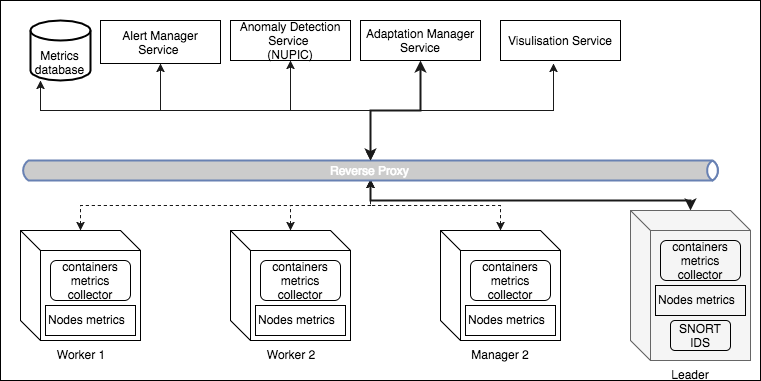
\includegraphics[scale=0.4]{design}
\caption{Microservices Architecture implemented in Docker Swarm}
\label{fig_model}
\end{figure*}


The prototype offering the architecture with the following functionality. \textbf{Metric collection}: Continuous collection of fine-grained metrics about cluster nodes, services, and containers including (CPU usage, Memory, Disk Reads Bytes/sec, Network Read/s, network write/s and Disk Writes Bytes/sec). The data are streamed into anomaly detection service. 

\textbf{Model Training}: The second step is to run NUPIC anomaly detection algorithm over the streamed data collected in Step 1. This will generate a model that will be used to detect anomaly for each metric selected in Step 1. 

\textbf{Anomaly Detection}: This component is responsible for running unsupervised machine learning algorithm based on NUPIC framework \cite{AHMAD2017134}. The collected real-time data is feed on the fly to NUPIC machine learning algorithm, which provides two features: first, contentious detection of anomalous behaviour with high accuracy. second, it also provide predictions about the architecture performance based on the collected historic data. This can alerts the architecture about incoming spike on resources demand which can be used by the adaptation manager to schedule a proactive adaptation strategy ahead of time. As shown in Figure \ref{fig_model}. The output of anomaly detection service is predictions, anomaly score and anomaly likelihood. 

\textbf{Adaptation Election}: Once their is an anomalous behaviour detected with high anomaly score and likelihood. The Alert manager will notify the adaptation manager about the context changes. The adaptation manager selects the adaptation action(s) after calculating the utility value for all actions as explained below in equ. \ref{eq_1}. Then, the adaptation manager uses the input of the anomaly likelihood, architecture constraints (specified by the DevOp during deployment), and desired/predicted QoS to calculate the best variation of the adaptation that has the highest utility. 

In different words, the DevOps define the policy parameters that suits the Microservices architecture, but the adaptation manager at runtime adjusts those polices based on the demand and the runtime requirements. The adjustment of the adaptation policy is a major challenge as there might a finite set of configurations and parameter tuning over unlimited number of contextual conditions. For this aim, the adaptation manager extended a multidimensional utility function described in \cite{KonstantinosKakousis:2008ub} to elect the best adaptation strategy. In this case, the adaptation strategy refers to any parameter-based or compositional-based configuration of the architecture, maintaining its original functional properties \cite{KonstantinosKakousis:2008ub}. The adaptation manager uses a utility function to calculate and priorities the requirements that need to be meet in the adaptation action. The adaptation manager provides continuous monitoring and detecting of the operational environment. Once an alert is triggered, the adaptation manager calculates the utility function for all metrics collected from the cluster's operational environment. 
From utility theory, a von Neumann-Morgenstern utility function $U_{i} : X_{i} \rightarrow \mathbb{R}$ 
assigns a real number to each quality dimension i, which we can normalize to the range [0, 1] \cite{fishburn1979two}. Across multiple dimensions of contextual changes, we can attribute a percentage weight to each dimension to account for its relative importance compared to other dimensions. These weights form the utility preferences. The overall utility is then given by the utility preference function calculated using equ. \ref{eq_1}. 

\begin{equation}
\label{eq_1}
fitness_{i}(V_{j},C_{m}) = \sum_{i}^{k} W_{i} U_{i}
\end{equation}

For example, if three objectives, u1, u2, u3, are given decreasing importance as follows: the first is twice as important as the second, and the second is three times as important as the third. Then the utility fitness would be quantified as $[w1 : 0.6, w2 : 0.3, w3 : 0.1]$. 
As soon as there is contextual changes detected in the architecture, the adaptation manager computes the utility of all variants related to the operational conditions and decides if an adaptation is required or not. This is achieved by checking if the current variant is still the one offering the highest utility or the predicted/desired variant of adaptation would offer higher utility. So, the utility function is calculated as in equ. \ref{eq_2} proposed in \cite{KonstantinosKakousis:2008ub}. 

Konstantinos et al. \cite{KonstantinosKakousis:2008ub} refer by the weight $W_{i}$ as the user preferences. In this paper we refer to $W_{i}$ as the anomaly likelihood calculated by NUPIC. This enables the adaptation manager to scale the weight of each context change over the distribution value calculated and aggregated by the anomaly likelihood in a scale between 0 to 1. Meaning if the $w_{i}$ for a metric like \textit{CPU Usage} is 1 and the CPU usage value is 70\% then this will give this metric high utility to be considered for the next adaptation action. 

The cost utility of provisioning a new node/container in the architecture is calculated based on the equ. \ref{eq_3}, where the $currentMetricValue_{i}$ is the current value of the context change, for example Memory ideal, $PredictedMetricValue_{i}$ refers to the Predicted value of the metric given by the NUPIC algorithm, $AnomScore_{i}$ is the Anomaly Score calculated by NUPIC at that point of time $t_{i}$, and $W_{i}$ is the weight calculated by the anomaly likelhood for the metric. The $UsageTime_{i}$ refers to the total number of hours the instance is expected to be used per/day, this value is calculated based on the rate of changes calculated based on equ. \ref{eq_4}. The $Cost_{i}$ is the cost in \$ for provisioning an instance per/day, normally this is a constant value specified by the cloud infrastructure provider based on the instance type.

\begin{equation}
\label{eq_2}
    Utility(V_{j},C_{m}) \equiv \frac{ \sum_{i=1}^{k} (W_{i} \cdot fitness_{i}(V_{j},C_{m}) ) }{\sum_{i=1}^{k} W_{i}}
\end{equation}

\begin{equation}
\label{eq_3}
 U_{i} = \frac{(currentMetricValue_{i} - PredictedMetricValue_{i})\cdot (AnomScore_{i} \cdot W(U_{i})}{UsageTime_{i} * Cost_{i}}
\end{equation}


 \begin{equation}
\label{eq_4}
\Delta U_{i}=\sum_{i}^{k} (U_{i}\cdot W_{i})-(U_{i-1}\cdot W_{i-1}
\end{equation}


\textbf{Adaptation Execution}: The adaptation manager executes the strategies based on the aggregated value of the utility function calculated in \ref{eq_2}. Once the adaptation action is completed by the adaptation manager, a set of adaptation actions are deployed in the architecture. To avoid, conflicts between multiple adaptation variations, the adapter allow the adaptation actions to be fully completed and verified by the cluster leader, then it will put a cool off timer before initiating new adaptation actions. This technique is used to avoid resources thrashing and preserving the cluster state for auto-recovery. The adaptation manager sends the cluster leader a set of instructions that might involve tuning of Microservice parameters like (CPU, Memory, Disk space, Network bandwidth), or vertical scaling of the Microservices containers like scaling a service in/out. In different scenarios and based of the calculation of the utility function, the adaptation action might involve horizontal scaling like add/remove nodes, add/remove managers, promote/demote nodes role as manager or worker. 

\textbf{Adaptation Verification}: The cluster leader and all managers in the cluster will vote on the adaptation action based on the consensus algorithm \cite{ongaro2015raft}. The vote results is used to to validate and verifies the adaptation action. If the adaptation action won the votes, the adaptation action will be executed by the cluster leader. If the adaptation action lost the vote, then the adaptation manager will re-initialised a new adaptation cycle.   
 
The evaluation of this model will come in two folds: First, evaluating the accuracy of the anomaly detection algorithms using confusion matrix \cite{kohavi1998confusion}.
Second, evaluating the constancy of the adaptation action and evaluating the state of the swarm after executing a set of adaptation actions as described in the following section. 

\section{Results} 
\label{sec:evaluation}
The swarm currently offers many services including the adaptation manager, which contains the NUPIC machine learning and the adaptation executer. This snapshot \footnote{https://goo.gl/LJPrFy} provides a full virtualisation and analytic of all services running in the swarm. The evaluation of the effectiveness of this model will be based on calculating a utility function for all metrics monitored, then it will calculates the number of adaptation attempts, successful convergence of services/nodes, or errors which leads to unstable state of the cluster. 

For this aim, first we run a stress test in the cluster manager until its CPU reaches 70\%, which triggers an alert to the adaptation manager. The adaptation manager collects the current reading of the metrics, anomaly score, and anomaly likelihood (see figure \ref{fig_model}). Then, the adaptation manager calculates the rate of changes in each metric to elect the metric that has the highest utility. As example, Figure \ref{fig_demand} is showing the utility of CPU usage (Uc), Memory usage (Um), Disk reads (Udr), Disk writes (Udw), Docker Network (Udn). The CPU usage has the highest utility as confirmed by the Utility indifference indicator shown in Figure \ref{fig_demand}. Also, the memory usage of the service shows slow rate of changes over time, which make it optional for the adaptation action. With regard to the utility of Disk Read/Write, the Figure \ref{fig_demand} shows no divergent above the moving average so it will not be considered in the next adaptation action. The docker network shows no changes over the time of the experiment as the load balancer and the reverse proxy diverted the traffic to many containers distributed in the cluster. 

As the $Utility_(CPU)$ has the highest value of changes as shown in Figure \ref{fig_demand}. This will triggers an adaptation action to reason about the high demand of CPU usage, so the adaptation manager will create additional nodes and join them to the swarm cluster automatically. The number of nodes is equals to the cost utility calculated as in equ. \ref{eq_4}. This results in adding new nodes to the swarm as shown in the snapshot \footnote{goo.gl/pGVmwZ} (A full visualised and analytics dashboard of the swarm after the adaptation).
Once the CPU demand is reduced, the adaptation manager will calculate the variations of the utility and remove number of nodes equals to value returned by the cost utility function in equ. \ref{eq_4}. A snapshot \footnote{https://goo.gl/H5js2s} of the system after the executing the adaptation action. 
\begin{figure*}[ht!]   
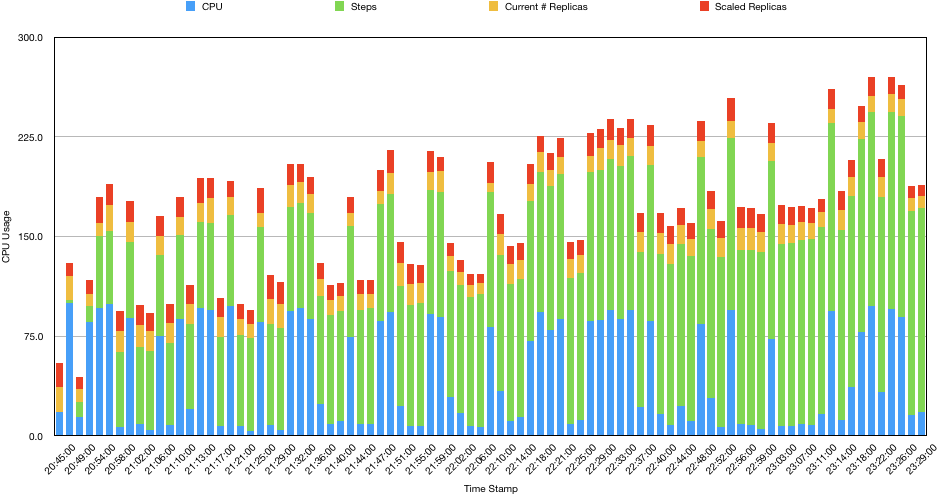
\includegraphics[scale=0.38]{ScalingService}
\caption{ Dynamic Scaling of Web Service}
\label{fig_Scale}
\end{figure*} 


\begin{figure*}[ht!] 
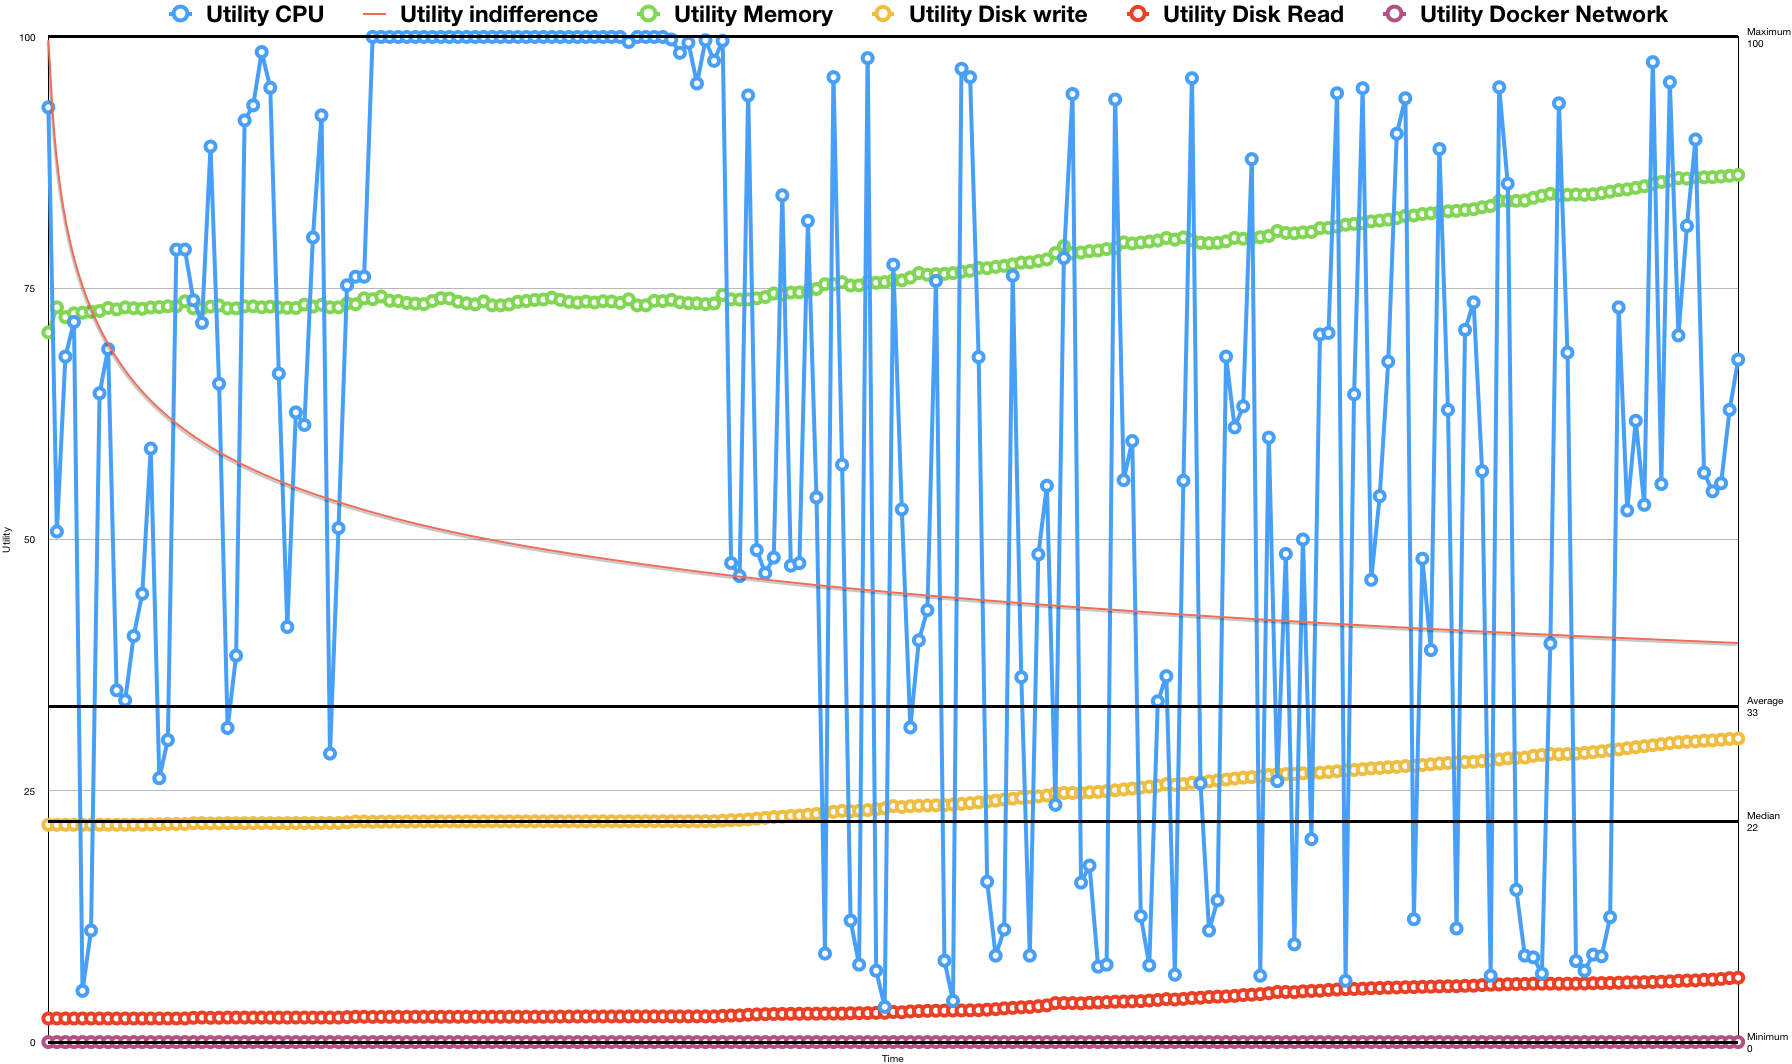
\includegraphics[scale=0.3]{demand}
\caption{ Dimensional analysis of variations of utility functions}
\label{fig_demand}
\end{figure*}
 \section{Discussion}
\label{sec:disc}

In another scenario, we simulated Distributed Denial of Service attack to a web service running in the swarm, to verify that the adaptation manager will be able to accommodate the DDOS by adding more replicas to the service. In this case, we wish to verify the ability of the proposed model to dynamical adjust the number of service's replicas against the variations of the CPU usage and to maintain an acceptable response time of the web service. At the same time, it is very important that the adaptation action would not scale the service endlessly. So the cost utility is calculated to count the number of replicas needed. The outcome of this experiments is shown in Figure \ref{fig_Scale}. The figure show how the number of scaled replicas are tuned linearly against the CPU usage. Also, it shows the number of steps taken by the adaptation manager to execute the scaling policy in/out. The adaptation manager counts the utility of the CPU metric and the cost utility to define the number of added/removed replicas. The adaptation manager waits for receiving a high utility value by sending heartbeat signal to get the latest value of utility and cost every 20s for a window of the 300s. Once the utility of the CPU elected, the adaptation manager calculates the number of replicas to be added/removed to the service. Also, the number of steps needed to achieve the desired state are counted as show in Figure \ref{fig_Scale}. The number of steps needed to perform the adaptation varies as its based on the severity and variation of the utility function over time. Once the adaptation is applied and verified by winning the consensus algorithm votes, the service will be scaled and the adaptation manager puts a cool off timer of 300s before initiating new adaptation action. Also, it reset the steps timer. The accuracy of the anomaly score and likelihood plays an important role for the successes this proposed model. 

One of a famous technique for evaluating anomaly detection algorithm is the use of a confusion matrix \cite{kohavi1998confusion}. The confusion matrix represents the total number of records inspected by algorithm as shown in Table \ref{Table_1}. The matrix represents the relationship between the actual levels of normal behaviour and the detected level of normal behaviour by the algorithm. Also, it represents the relationship between the actual anomaly recorded in the system and the predicted/identified anomaly that the algorithm identified as anomalous behaviour.   

In case of our proposed model, If NUPIC anomaly detection considered a specific record as anomalous and it was an actual anomaly then this attempt is classified as a \textbf{True Positive}. If NUPIC classifies the data as normal behaviour and it was normal data then this attempt is classified as \textbf{True Negative}. If NUPIC classifies an anomalous behaviour as normal behaviour this means that NUPIC failed to detect anomaly. In the case, this attempt is classified as \textbf{False Negative}. If NUPIC classifies the data as anomalous behaviour but the data was normal behaviour then this attempt is considered a False Alarm/\textbf{False Positive}. Both True Positive and False Positive are important benchmark to measure the accuracy of intrusion detection systems. Table \ref{Table_1} summarizes the values used for evaluating the anomaly detection algorithm we used in this paper. The confusion matrix will be used to calculate the model detection rate, false positive, and accuracy. Those results will be compared against SNORT \footnote{https://snort.org} \cite{roesch1999snort}. SNORT is implemented in as a container in the leader node.(see Figure \ref{fig_model}). Based on the calculations of NUPIC anomaly detection shown in Table \ref{Table_1} and Snort in Table \ref{Table_2}, it was found that our proposed model of using NUPIC performs significantly better in terms of the detection rate, false alarms, and accuracy. The false alarm rate in the model (0.0264) is lower than SNORT (1,12). In addition, the model provides a high rate of true alarms and anomaly detection as summarised in Table \ref{Table_3}. The equations used in this evaluation are listed in \ref{Table_3}.    
 
\begin{table}[h!]
\centering

\caption{Results of the proposed anomalies detection model on confusion matrix}
\resizebox{\columnwidth}{!}{ 
\label{Table_1}
 \begin{tabular}{|c|c|c|}
        \hline
        X= 1528   & Predicted anomalies & Predicted normality \\
        \hline
        Actual anomalies (TP + FN) (55) & TP = 49   & FN = 6 \\
        \hline
        Actual normalies (FP + TN) (1473)& FP/ False Alarm = 38 & TN = 1435   \\
        \hline
        \end{tabular}
}
\end{table}

 
 \begin{table}[h!]
\centering

\caption{Results of the SNORT anomaly detection on confusion matrix}
\resizebox{\columnwidth}{!}{ 
\label{Table_2}
 \begin{tabular}{|c|c|c|}
        \hline
        X= 1528   & Predicted anomalies & Predicted normality \\
        \hline
        Actual anomalies (TP + FN) (55) & TP = 32   & FN = 23 \\
        \hline
        Actual normalies (FP + TN) (1473)& FP/ False Alarm = 62 & TN = 1411   \\
        \hline
        \end{tabular}
}
\end{table}

 
 



\begin{table}[h!]
\centering
\footnotesize
\caption{Comparison between SNORT Anomaly Detection and the Proposed Model}
\label{Table_3}
\begin{tabular}{|p{2cm}|c|c|p{4cm}|}
 \hline 
 Rate & NUPIC & SNORT & Result \\ 
 \hline 
 Accuracy  & 0.97 & 0.944 &  Implementation of NUPIC provides better accuracy $Accuracy=(TP+TN)/x$, over the SNORT anomaly detection. \\ 
 \hline 
 Misclassification  & 0.0287 & 0.0554 & The rate of false alarms is lower in the proposed model compared with SNORT. The Misclassification is calculated using $Misclassification=(FP+FN )/x$ \\ 
 \hline 
 True Positive Rate (TP)  & 0.89 & 0.58 & $TP\;rate=TP/(Actual\;anomalies\;in\;x)$. The rate of true alarms in the model is significantly better than SNORT. \\ 
 \hline 
 False Positive (FP)/ False Alarm & 0.0264 & 1.12 & The proposed model has a lower rate of incorrect classification of attacks calculated using $FP \;rate =FP/(Actual\;in\;x)$, but SNORT has a higher rate of not detecting attacks and considering them as normal behaviour \\ 
 \hline 
 True Negative (TN & 0.998 & 0.981 & Both models- SNORT and the proposed model- have a good rate of detecting the normal behaviour of the system as calculated by $TN\;rate=TN/(Actual\;in\;x)$. However, the proposed model provides better results.  \\ 
 \hline 
 Precision  & 0.89 & 0.58 & The precision $Precision=TP/(Predicted\;anomalies\;in\;x)$, of the proposed model is far better than SNORT. The gap between the two models is clear. \\ 
 \hline 
 Prevalence  & 0.03599 & 0.03599 & Both models have the same prevalence rate calculated by $Prevalence=(Actual\;anomalies)/x$ as the DDOS was simulated as part of the experiment. \\ 
 \hline 
 
 \end{tabular} 
\end{table}
 The values in Table \ref{Table_3} clearly show that the proposed model performs better in terms of false alarms, detection rate, and accuracy. A further calculation, as shown below, could provide a better idea of the performance of the proposed model. The detection rate of SNORT is $32/((32+62) )=0.340$ and this indicates that the proposed model has a better detection rate, as the proposed model used a machine-learning algorithm to build a model about the data and provides a prediction for each value. Those factors improve the detection rate compared with SNORT, which used a rule-based engine to match the incoming traffic and pre-configured rules. 

The False Alarm of the proposed model  is $0.0257$. This indicates that the proposed model has a very low rate of providing a false alarm or identifying normal behaviour as anomalous. In the contrast, the false alarm for SNORT is $62/((62+1411))=0.042$. This value is a clear indication that SNORT would provide more false alarms about normal traffic in the system. This is due to the fact that SNORT considers one factor of identifying an anomaly which is the network traffic. In contrast, the proposed model continuously observed and learned the behaviour of so many performance criteria about the cluster in addition to the network traffic. 

The overall accuracy of the proposed model is $0.97$. The accuracy of SNORT is 0.944, due to the fact that SNORT is continuously monitoring the system network, but it has no means of understanding the behaviour of the system. The proposed model builds an accurate model of the system behaviour so it has better insight into any fluctuations or spikes in the data. This feature is considered very important for the success of the adaptation strategy and the self-healing property of the Microservices architecture. However, we believe that this model manages to offer the Microservices architecture with continuous monitoring, continuous detection of anomalous behaviour, and provides the architecture with dynamic decision making based on the employment of multidimensional utility-based model. The results in above, shows high accuracy in detecting the anomaly and an accurate calculation of variant adaptation actions. It Also shows high success rate in performing horizontal and vertical autoscaling in response to contextual changes. 

 


 \section{Conclusions and Future Work}\label{sec:Conclusion}
 Anomaly Detection using statistical approaches are not suitable for Microservices Architecture. It is difficult to determine the thresholds of a virtualised resources, which can be used to perform scaling or configuration policies. 
Also, it is difficult to have an accurate profile of Microservices cluster that has an accurate distribution among all measures found in the cluster. Real-time data streams introduces big challenges for machine learning algorithms as data streams are often found with massive volumes and high velocities. 

Finally, this paper provides an architecture model that guarantees a continuous monitoring and observing of Microservices architecture. Also, it employs a mechanism for real-time unsupervised anomaly detection algorithm, which offers high accuracy of detecting normal and abnormal behaviour of the architecture. The uses of utility functions enables the architecture to dynamically elect a reasoning approach based on the utility of the changes in the operational environment.
The self-healing property is achieved by parameter tuning of the running services and dynamic adjustment of the cluster nodes. We believe integrating utility theory in the decision making process improves the effectiveness of the adaptation and reduces the adaptation risk including resources over-provisioning and thrashing. Also, it preserving the cluster state by preventing multiple adaptation to take place at the same time. Enabling a prediction over the metrics of the operational resources enables the architecture to schedule a proactive adaptation actions. 
This model requires further improvement with regard to services compositions, and decentralised decision making. A complete decentralisation of the adaptation manager, as it is currently implementing the adaptation manager as central component in the leader node. Also, this model requires an enhanced mechanism of run-time configurations, as it support at the moment parameter tuning of the architecture configuration. Also, the current implementation of NUPIC requires multiple implementations for each contextual changes. NUPIC has no support for swarming over multiple variables data model. Finally, we believe the ability of the Microservices to self-heal itself is achievable, but a major question stand related to how we could evaluate the self-healing property of Microservice architecture. This question require further investigation to find applicable runtime evaluation mechanisms      

\bibliographystyle{ACM-Reference-Format}
\bibliography{selfhealingv2.bib} 

\end{document}
    